\section{Tema 4: Conservación de la cantidad de movimiento}
\subsection{Teorema del transporte de Reynolds para la cantidad de movimiento}
Sea un volumen sometido a un conjunto de fuerzas:
\begin{figure}[H]
	\centering
	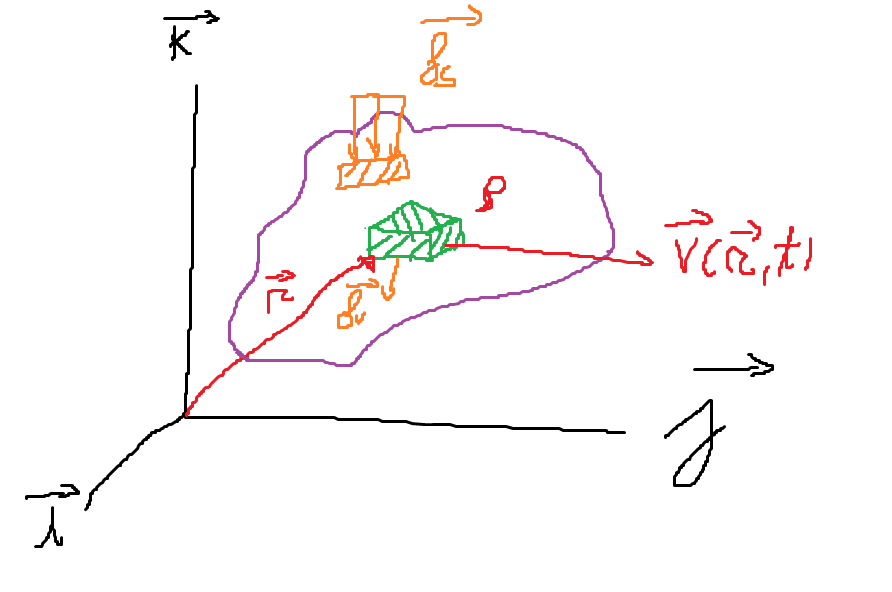
\includegraphics[width=0.7\linewidth]{imagenesTema4/magnitudesFuerzas}
	\caption{Magnitudes principales que influencian la cantidad de movimiento.}
	\label{fig:magnitudesfuerzas}
\end{figure}

Aplicando al teorema del transporte de Reynolds la función $\Phi=\rho\vec{v}$ y una similitud con la segunda ley de Newton se obtiene para volúmenes fluidos:
\[\iiint_{V_f}\vec{f}_V\,dV+\oiint_{S_f}\vec{f}_s\,dS=
\frac{d}{dt}\iiint_{V_f}\rho\vec{v}\,dV=
\iiint_{V_f}\frac{\partial \rho\vec{v}}{\partial t}\,dV+\oiint_{S_f}\rho\vec{v}\left(\vec{v}\cdot\vec{n}\right)\,dS\]

Para un volumen de control:
\[\iiint_{V_f}\vec{f}_V\,dV+\oiint_{S_f}\vec{f}_s\,dS=
\frac{d}{dt}\iiint_{V_f}\rho\vec{v}\,dV=
\iiint_{V_c}\frac{\partial \rho\vec{v}}{\partial t}\,dV
+\oiint_{S_c}\rho\vec{v}\left[\left(\vec{v}-\vec{v}_c\right)\cdot\vec{n}\right]\,dS\]

En estas expresiones aparecen dos tipos de fuerzas:
\begin{enumerate}
	\item Fuerzas volumétricas $\vec{f}_v$
	\begin{enumerate}
		\item Típicamente son fuerzas relacionadas con campos:
		\[\vec{f}_v=\rho \vec{g}\]
		\item Pueden ser también fuerzas de inercia en sistemas de referencia móviles.
	\end{enumerate}
	\item Fuerzas superficiales $\vec{f}_s$
	
	\begin{enumerate}
		\item La expresión general de estas fuerzas es:
		\[\vec{f}_s=
		\red{\underbrace{\black -P\vec{n}}_{\text{Presión hidroestática}}}\black
		+
		\red{\underbrace{\black \overline{\overline{\tau}}_v\cdot\vec{n}}_{\text{Esfuerzos viscosos}}}\black
		\]
		\item Siendo el tensor de esfuerzas viscosos (es una ecuación constitutiva, depende del material):
		\[
		\overline{\overline{\tau}}=
		\begin{bmatrix}
			\tau_{xx} &\tau_{xy} & \tau_{xz} \\
			 \tau_{yx}&  \tau_{yy}& \tau_{yz}\\	
			\tau_{zx} & \tau_{zy} & \tau_{zz} \\
		\end{bmatrix}
		=2\mu \overline{\overline{\xi}} + \lambda \left(\vec{\nabla}\cdot \vec{v}\right)\overline{\overline{I}}
		\]
		Donde \begin{itemize}
			\item $\mu$ es la viscosidad.
			\item $\lambda$ es la viscosidad volumétrica.
			\item $\overline{\overline{I}}$ es la matriz identidad.
		\end{itemize}
	\end{enumerate}
\end{enumerate}
\subsection{Ecuaciones de Navier-Stokes}
Se parte del teorema del transporte de Reynolds:
\begin{equation}
\iiint_{V_f}\vec{f}_V\,dV
+
\oiint_{S_f}\vec{f}_s\,dS
=
\iiint_{V_f}\frac{\partial \rho\vec{v}}{\partial t}\,dV
+
\oiint_{S_f}\rho\vec{v}\left(\vec{v}\cdot\vec{n}\right)\,dS
\end{equation}
Desarrollando mediante el teorema de la divergencia de Gauss:
\begin{equation}
	\oiint_{S_f}\vec{f}_s\,dS
	=
	\oiint_{S_f}-P\vec{n}_s\,dS
	+
	\oiint_{S_f}\overline{\overline{\tau}}\cdot\vec{n}_s\,dS
	=
	\iiint_{V_f}-\vec{\nabla}p\,dV
	+
	\iiint_{V_f}\vec{\nabla}\cdot\overline{\overline{\tau}}\,dV
\end{equation}

\begin{equation}
\oiint_{S_f}\rho\vec{v}\left(\vec{v}\cdot\vec{n}\right)\,dS
=
\iiint_{V_f}\vec{\nabla}\cdot\left(\rho \vec{ v} \otimes \vec{v}\right)\,dV
\end{equation}

Juntando las ecuaciones (5), (6) y (7):
\[\iiint_{V_f}\vec{f}_V\,dV
+
\iiint_{V_f}-\vec{\nabla}P\,dV
+
\iiint_{V_f}\vec{\nabla}\cdot\overline{\overline{\tau}}\,dV
=
\iiint_{V_f}\frac{\partial \rho\vec{v}}{\partial t}\,dV
+
\iiint_{V_f}\vec{\nabla}\cdot\left(\rho \vec{ v} \otimes \vec{v}\right)\,dV
\]

Para un valor $V_f \approx dV$ arbitrariamente pequeño pero no nulo. Se obtiene la ecuación Navier-Stokes en forma conservativa:
\[
\vec{f}_V
-
\vec{\nabla}P
+
\vec{\nabla}\cdot\overline{\overline{\tau}}
=
\frac{\partial \rho\vec{v}}{\partial t}
+
\vec{\nabla}\cdot\left(\rho \vec{ v} \otimes \vec{v}\right)
\]

Desarrollando:
\[\vec{f}_V
-
\vec{\nabla}P
+
\vec{\nabla}\cdot\overline{\overline{\tau}}
=
\red{\underbrace{\black \rho\frac{\partial\vec{v}}{\partial t}
+
\rho \left(\vec{v}\cdot\vec{\nabla}\right)\vec{v}}_{\rho\frac{D\vec{v}}{Dt}}}\black\]
\[\vec{\nabla}\cdot\overline{\overline{\tau}}
=
\vec{\nabla}\cdot\left(2\mu\overline{\overline{\xi}}\right)
+
\vec{\nabla}\cdot\left[\lambda\left(\vec{\nabla}\cdot\vec{v}\right)\overline{\overline{I}}\right]
=
\vec{\nabla}\cdot\left(2\mu\frac{\vec{\nabla}\vec{v}+\left(\vec{\nabla}\vec{v}\right)^T}{2}\right)
+
\lambda\vec{\nabla}\cdot\left[\left(\vec{\nabla}\cdot\vec{v}\right)\overline{\overline{I}}\right]
\]

\[\vec{\nabla}\cdot\overline{\overline{\tau}}
	\stackrel{\mu,\lambda=cte}{=}
	\mu\vec{\nabla}^2\vec{v}+\left(\mu+\lambda\right)\vec{\nabla}\left(\vec{\nabla}\cdot\vec{v}\right)
	\]
	
En fluidos newtonianos se cumple que $\rho,\mu=cte$ con lo cual:
\[\frac{\partial \rho}{\partial t}=0; \vec{\nabla}\rho=0; \vec{\nabla}\cdot\vec{v}=0\]

Por tanto, las ecuaciones de Navier-Stokes junto a la conservación de la masa en forma diferencial:
\[\rho\frac{\partial \vec{v}}{\partial t}+\rho\left(\vec{v}\cdot\vec{\nabla}\right)\vec{v}=-\vec{\nabla}P+\mu\vec{\nabla}^2\vec{v}+\rho \vec{g}\]
\[\frac{\partial \rho}{\partial t} +\vec{\nabla}\cdot\left(\rho\vec{v}\right)=0\]
\subsection{Número de Reynolds}
El número de Reynolds es un número adimensional que se emplea para caracterizar el movimiento de un fluido y se define como:
\[Re=\frac{\text{Orden de magnitud de la inercia convectiva}}{\text{Orden de magnitud de fuerzas viscosas}}\]
\[Re=\frac{|\rho\left(\vec{v}\cdot\vec{\nabla}\right)\vec{v}|}{|\mu\vec{\nabla}^2\vec{v}|}
\stackrel{|\vec{\nabla}|=\frac{1}{L_c}}{=}\frac{\rho_c v^2_c/L_c}{\mu_c v_c/L^2_c}=\frac{\rho_c v_c L_c}{\mu_c}\]
\begin{itemize}
	\item Si Re es elevado, el flujo es de inercia dominante, flujo turbulento.
	\item Si Re es bajo, el flujo es de viscosidad dominante, flujo laminar.
\end{itemize}
\subsection{Teorema de Bernouilli}
Se parte de la ecuación de Navier-Stokes en forma diferencial:
\[\rho\frac{\partial \vec{v}}{\partial t}+\rho\left(\vec{v}\cdot\vec{\nabla}\right)\vec{v}=-\vec{\nabla}P+\mu\vec{\nabla}^2\vec{v}+ \vec{f}_v\]

Desarrollando:
\[\rho\frac{\partial \vec{v}}{\partial t}
+
\rho\vec{\nabla}\frac{|\vec{v}|}{2}^2-\rho\vec{v} \times \left(\vec{\nabla}\times\vec{v}\right)
=-\vec{\nabla}P+\mu\vec{\nabla}^2\vec{v}+\vec{f}_v
\]

Se supone un líquido incompresible, estacionario, fuerzas de viscosidad despreciables y que las fuerzas volumétricas tienen la siguiente función potencial:
\[\vec{f}_V=-g\vec{\nabla}U_g\]
\[\rho\vec{\nabla}\frac{|\vec{v}|}{2}^2
-
\rho\vec{v} \times \left(\vec{\nabla}\times\vec{v}\right)
=
-\vec{\nabla}\left(P+\rho U_g\right)\]

Multiplicando por $\vec{v}$
\[\vec{v}\cdot\left[\rho\vec{\nabla}\frac{|\vec{v}|}{2}^2
-
\rho\vec{v} \times \left(\vec{\nabla}\times\vec{v}\right)
=
-\vec{\nabla}\left(P+\rho U_g\right)\right]\rightarrow\vec{\nabla}\left(P+\frac{1}{2}\rho|v|^2+\rho U_g\right)=0\]

De esta expresión se deduce que:
\[P+\frac{1}{2}\rho|v|^2+\rho U_g=cte\]

En el caso de que el campo potencial gravitatorio sea paralelo al eje z, se obtiene el teorema de Bernouilli:
\[P+\frac{1}{2}\rho|v|^2+\rho gz=cte\]